\chapter{Análisis espectrales: resultados numéricos}
\label{chap: resultados numericos analisis espectrales}

Después de todo lo expuesto en las secciones anteriores, tenemos
ya dos alternativas para graficar el espectro
de una señal $x \in \IR^{n}$.

\begin{itemize}
	\item Usando la transformada discreta de Fourier
	(c.f. sección \ref{sec: TDF}), el espectro de
	una señal $x$ es la gráfica de las frecuencias
	enteras dadas (dependiendo de la 
	paridad de $n$) por las
	tablas 6.1 y 6.2
	versus los coeficientes
	$\tau_{n}(x)$ definidos en
	\ref{def: taus}.
	\TODO{Puesto que hacer un análisis con la
	DFT significa expresar a $x$ como una suma
	ponderada de muestreos de senos y cosenos
	de algunas frecuenicas enteras,...}
	
	\item Si, para hacer un análisis espectral, se usan
	las ideas propuestas en 
	la sección
	\ref{sec: metodologia para realizar un analisis espectral que considere frecuencias arbitrarias}, entonces, dado un rango de frecuencias 
	$\omega$,
	el espectro de $x$ es la gráfica de 
	las frecuencias $\omega$ versus	
	los coeficientes
	$\sigma_{n}(x, \omega)$.
	

\TODO{a diferencia de la dft, los casos extremos ya no son
estar o no estar, sino ser perpendicular o ser paralelo a su
representante del espacio monofrecuencial.}
\end{itemize}


\begin{figure}[H]
	\sidecaption{
	Ejemplo de los espectros resultantes
	de los dos métodos de análisis.
	\label{fig: espectro 1 }
	}
	\centering
	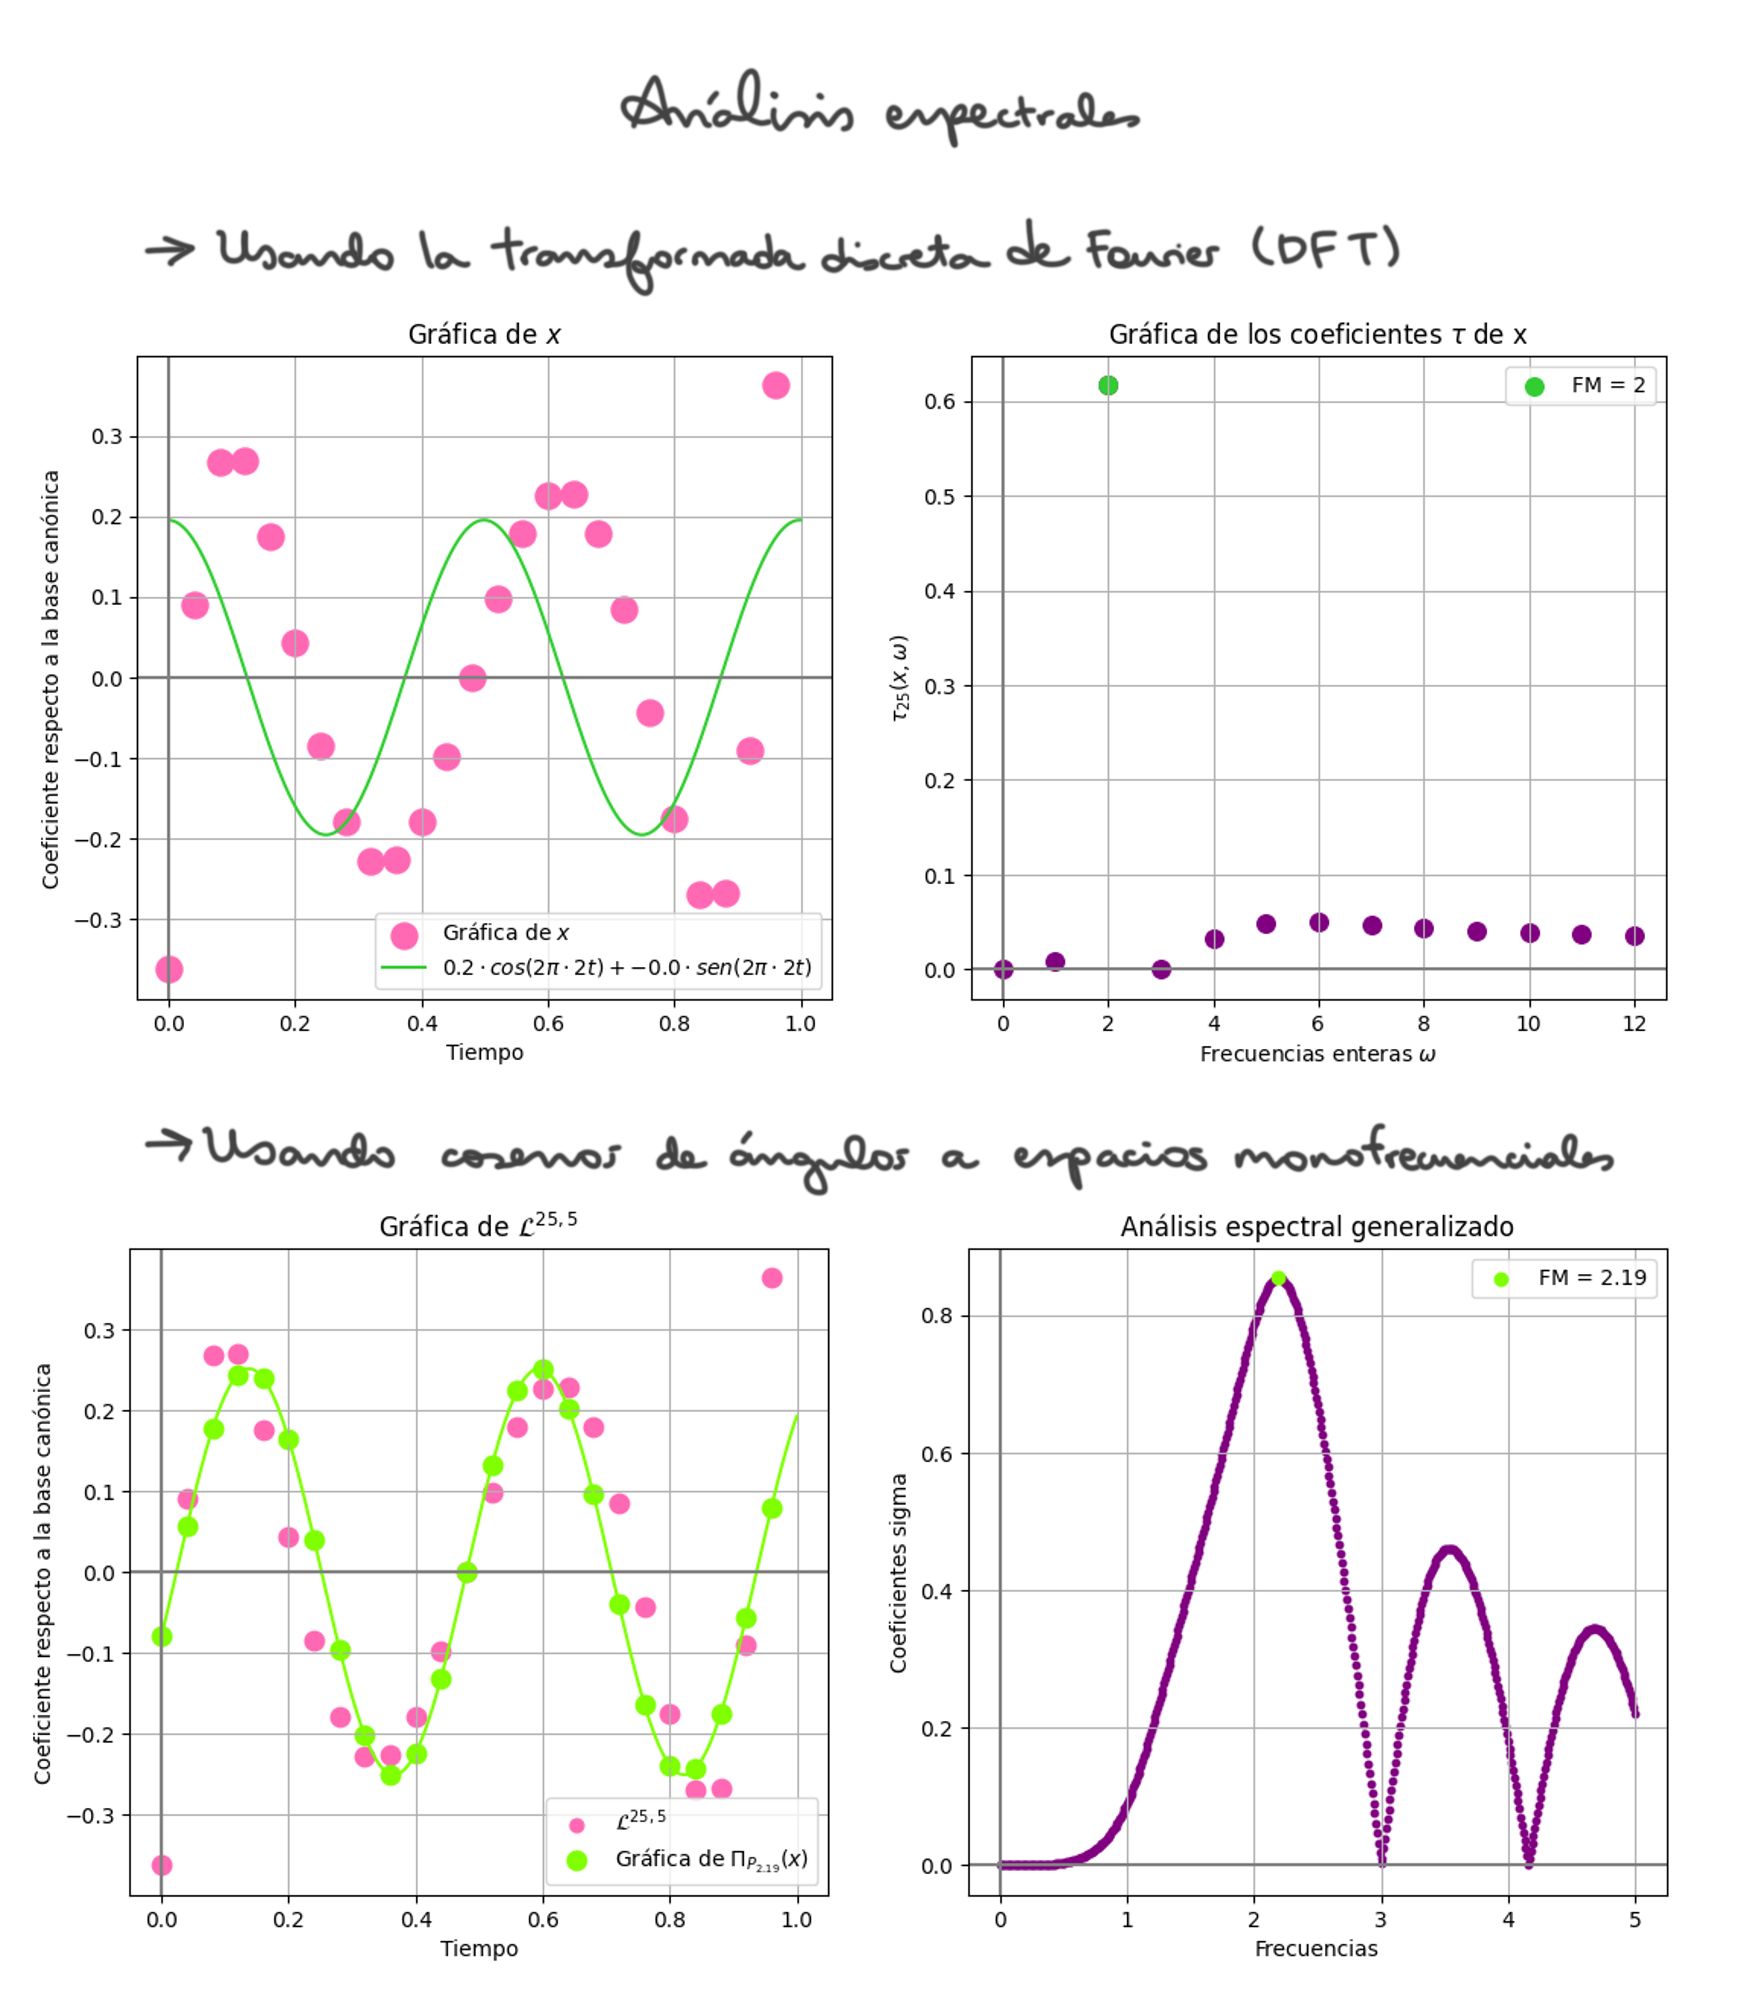
\includegraphics[scale = 1]{ejemplo_analisisEspectrales} 
\end{figure}	